\section{Event selection}
\label{sec:evtsel}

%The physics objects definition follows the recommendations of the CMS SUSY group Reference Analysis, for the single-electron and muon channels, as proposed in \cite{}.
A ``single-lepton'' event is defined through a series of selection requirements on the basic physics objects, i.e. the electrons, muons, jets and the missing transverse energy. A concrete list of these requirements, including acceptance as well as identification (ID) and quality criteria, have been proposed by the Single-lepton Reference Analysis (RA4) \cite{ra4}. In this Note, we follow the guidelines proposed in RA4, while for some specific selection requirements we investigate possible changes which improve the analysis within the context of usage of the $\alpha_{T}$ variable to control the QCD background. The main modifications with respect to the RA4 guidelines are the lowering of the lepton momenta (down to 5 GeV threshold) as well as a redefinition of the lepton isolation -- applicable to a soft lepton selection.

\subsection{Single-lepton Reference Analysis (RA4) baseline}

The RA4 selection \cite{ra4} has been proposed to provide a baseline selection in the single-lepton mode SUSY searches for CMS. It was not intended to be, and nor is it currently, the most optimal choice of the selection requirements.  Nevertheless, it provides a reference to all possible analysis strategies to start with. In the current analysis, we adopt the following definition of physics objects from RA4:

\begin{description}
\item[Electron selection:] Electron objects are reconstructed with the PixelMatchGsfElectron algorithm whereas the ID imposed is the ''IdRobustLoose'' cut-based identification requirement \cite{elecid}. The electron transverse momentum is required to be above 10 GeV and the $\eta$-acceptance is $|\eta|<2.4$. There is also a cut on the impact parameter ($d_{0}$) of the electron track in order to eliminate electrons which are incompatible with the primary vertex (PV): $|d_{0}| < 0.2$ is imposed.

\item[Muon selection:] Muon objects are ``global muons'', which are provided by the best matching pair between a ``standalone-muon track'' and charged-particle tracks reconstructed in the inner tracker system (``tracker-tracks''). For each pair of such tracks, a combined fit using all hits in both tracks is performed based on the Kalman filter technique, in order to obtain the final ``global muon'' object. Global muons are required to satisfy the muon identification algorithm ``GlobalMuonPromptTight'' \cite{muonid}, which applies quality requirements to the muon tracks.  The muon transverse momentum is required to be above $10$ GeV and within $|\eta|=2.1$. A $\chi^{2}/Ndof < 10$ cut is further applied to the combined muon track, while the tracker track is required to have more than eleven (11) valid hits. As in the case of electrons, muons are required to be compatible with the PV, by applying $|d_{0}| < 0.2$.

\item[Jet selection:] Jet objects are identified starting from the CaloJet collection, produced with the ``IterativeCone5'' algorithm. The following selection criteria are applied; each jet must have $P_{T}>30$ GeV and $|\eta| < 3$. A quality requirement using the electromagnetic energy fraction (EMF) in the CaloJet, is applied as $EMF < 0.9$, in order to obtain the final ``good-jet'' object.

\item[Missing Transverse Energy (MET) selection:] The calorimeter missing energy (CaloMET) is determined from the transverse vector sum over energy deposits in projective Calorimeter Towers:
\begin{eqnarray}
%\not{\vec{E}_{T}} = - \sum_{n} ( E_{n} \sin \theta_{n} \cos \phi_{n} \hat{i} + E_{n} \sin \theta_{n} \sin \phi_{n} \hat{j} ) = \not{E_{x}} \hat{i} + \not{E_{y}} \hat{j}
\not{\vec{E}_{T}} = \not{E_{x}} \hat{i} + \not{E_{y}} \hat{j}
\end{eqnarray}
Further corrections on the calorimetric MET are applied to take into account the jet energy response (jet energy scale corrections), as well as the muon corrections.

\end{description}

\subsection{Lepton selection and isolation requirements}

Lepton isolation is a key tool in reducing backgrounds from fake or heavy-flavor electrons and muons -- collectively referred to as ``QCD sources'' in what follows. The standard recommendations for lepton isolation are provided by the V+jets Cross PAG group \cite{vjets}, and have been shown to work well for electrons and muons with momenta above $\sim$ 30 GeV. For lower lepton $p_{T}$, however, the standard isolation selection has a significant impact on the efficiency of both electrons and muons. For this reason, a different isolation is considered for leptons in the region $p_{T}^{\ell} < 30$ GeV (``soft lepton'' region). An optimization of the electron and muon isolation performance in the soft $p_{T}$ region has been developed elsewhere \cite{iso}. The isolation variables and the resulting cut values are optimized for optimal efficiency of SUSY signal leptons versus background rejection. 

The overall isolation requirements imposed to the electron and muon objects of the analysis are summarised in table \ref{tab:iso}. In the high $p_{T}$ region, electrons and muons are required to pass the combined relative isolation criterio according to the V+jets recommendations:
\bea
\textrm{CombIso}_{rel} = \frac{\sum_{\Delta R < 0.3} p_{T}^{\textrm{track}}}{p_{T}^{\ell}} +  \frac{\sum_{\Delta R < X} E_{T}^{\textrm{ECAL}}}{E_{T}^{\ell}} +  \frac{\sum_{\Delta R < Y} E_{T}^{\textrm{HCAL}}}{E_{T}^{\ell}}
\eea
where $\sum_{\Delta R < 0.3} p_{T}^{\textrm{track}}$ is the sum of the transverse momenta of the tracker-tracks in a cone ($\Delta R < 0.3$ for both electrons and muons) around the lepton direction. $\sum_{\Delta R < X} E_T^{\textrm{ECAL}}$ and $\sum_{\Delta R < Y} E_T^{\textrm{HCAL}}$ are the
sums of the energy deposits in a cone ($\Delta R < 0.3$ for muons and $\Delta R < 0.4$ for electrons) around the lepton direction in the electromagnetic and hadronic calorimeter respectively.

In the soft lepton $p_{T}$ region, we choose to use only the tracker based isolation since this is expected to perform more reliably at least for the early phase of the LHC operation. A cut on the absolute tracker isolation is set to $\sim$ 3 GeV for electrons and $\sim$ 5 GeV for muons:
\bea
\textrm{TrkIso}_{\textrm{abs}} = \sum_{\Delta R < 0.3} p_{T}^{\textrm{track}}
\eea

\begin{table}[h!]
\centering
\begin{tabular}{|c||c|c|}
\hline
$p_{T}$ region & Electron iso & Muon iso \\ \hline
``high'' ($p_{T}^{\ell} > 30 \textrm{GeV}$) & $\textrm{CombIso}_{\textrm{rel}} < 0.1$ & $\textrm{CombIso}_{\textrm{rel}} < 0.1$ \\ \hline
``soft'' ($5 < p_{T}^{\ell} < 30 \textrm{GeV}$) & $\textrm{TrkIso}_{\textrm{abs}} < 3 \textrm{GeV}$ & $\textrm{TrkIso}_{\textrm{abs}} < 5 \textrm{GeV}$ \\ \hline
%``soft'' ($5 < p_{T}^{\ell} < 30 \textrm{GeV}$) & $\textrm{TrkIso}_{\textrm{abs}} < 2. + 0.06 p_{T}^{\e}$ & $\textrm{TrkIso}_{\textrm{abs}} < 7. + 0.3 p_{T}^{\e}$ \\ \hline
\end{tabular}
   \caption{\textit{\small{Isolation requirements imposed to the electron and muon objects of the single-lepton analysis. The tracker absolute isolation is chosen for the ``soft lepton'' region, with a $p_{T}$-dependent cut value, and the relative combined isolation (V+jets cross PAG recommendation) is chosen in the ``high-$p_{T}$'' region.}}}
 \label{tab:iso}  
\end{table}

For purposes of the lepton isolation performance study, a lepton classification
tool based on Monte Carlo (MC) truth information was developed. Reconstructed electrons and muons were matched to
generator level leptons ($e$ or $\mu$'s), and assigned to a certain category according to the
generated lepton: i) ``Prompt'' leptons were identified as the ones originated by
the decay of a SUSY particle, a $W/Z$ or a $\tau$; 
ii) ``Heavy-Flavor''  originated from hadronic decays of heavy-flavor 
particles ($b/c$ decays); iii) ``Fake''  reconstructed leptons did not have any correspondent
lepton at the truth generated level. In the case of muons, the latter category
includes in-flight decays of $\pi/K$-mesons, as well as jet punch-through.


Matching between generated and reconstructed leptons was performed using a
cone in ($\eta, \phi$) plane. %phase space.
The distance between generated and reconstructed leptons,
$\Delta R = \sqrt{(\Delta \eta)^2 + (\Delta \phi)^2}$, was required to be less then 0.5, and the
closest generated lepton was associated with the corresponding reconstructed candidate. If no
generated lepton was found within the $\Delta R$ cone the reconstructed lepton was considered to be
a ``fake''. The leptons were reconstructed at detector level and passed identification
procedure as described in the previous subsection. Only electrons that satisfied RobustLoose and muons that satisfied
GlobalTight identification requirements were selected. Generated and reconstructed electrons were
required to have $p_{T} >$ 5~GeV and $|\eta| < 2.5$, muons, $p_{T} >$ 3~GeV  and $|\eta| < 2.1$. 

Lepton reconstruction and isolation efficiencies, defined as the ratio of the number of reconstructed and matched
leptons to the total number of generated leptons, were estimated for prompt leptons and leptons from heavy-flavor decays separately, using the SUSY
LM0 sample. The efficiency curves are presented in fig.~\ref{fig:ele-eff} for electrons and fig.~\ref{fig:muon-eff}
muons as a function of the generated lepton $p_{T}$. 

\begin{comment}
An additional ``isolation'' variable can be formed by the $\Delta R (\ell - \textrm{jet})$, which is the distance, in the eta-phi space, between the electron or muon and its closest (good) jet. This variable has been shown to be quite effective in reducing remaining background leptons in QCD events, and can be applied in order to complement the tracker and calorimeter isolation above. In the scope of this analysis, a separation between each electron or muon from a jet is imposed with the following veto requirement:
\bea
\Delta R(e - \textrm{jet}) > 0.5, \;\;\;\; \Delta R(\mu - \textrm{jet}) > 0.5
\eea			

The effectiveness of this veto is shown in table \ref{tab:drveto}, where the efficiency of the cut in the SUSY signal and all the SM background processes has been calculated. Overall, a lepton-jet separation rejects almost $\sim 50\%$ of the QCD events, while having a small impact on the SUSY signal efficiency.

\begin{table}[h!]
   \centering
\begin{tabular}{|c||c|c|c|c|c|c|}
\hline
& LM0 & LM1 & $t\bar{t}$ & $W$ & QCD & $b\bar{b}$ \\ \hline
$\Delta R(\mu-j) > 0.5$ & 0.13 & 0.09 & 0.13 & 0.05 & 0.45 & 0.42 \\ \hline
\end{tabular}
  \caption{\textit{\small{blabla}}}
  \label{tab:drveto}
\end{table}

\end{comment}

\begin{figure}[h!]
\begin{minipage}[b]{0.5\linewidth}
\centering
{\label{fig:lm1_cor}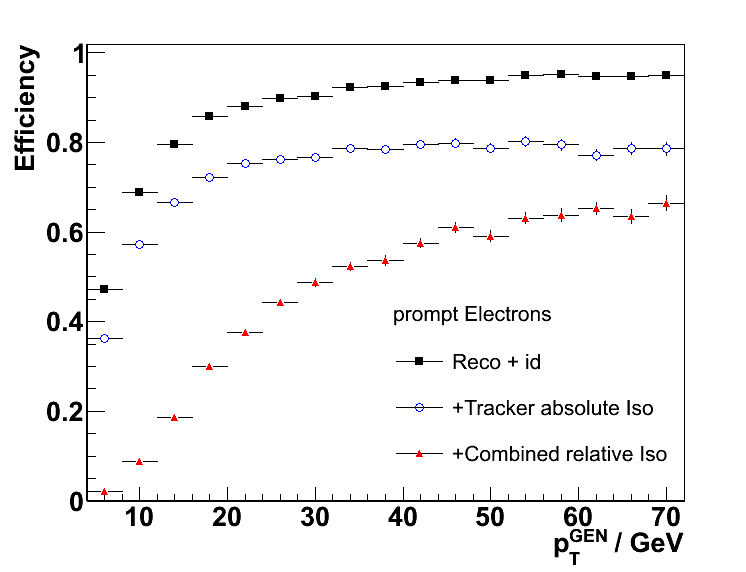
\includegraphics[scale=0.32]{./plots/prompt_ele_eff.png}}
\end{minipage}
\begin{minipage}[b]{0.5\linewidth}
\centering
{\label{fig:qcd_cor}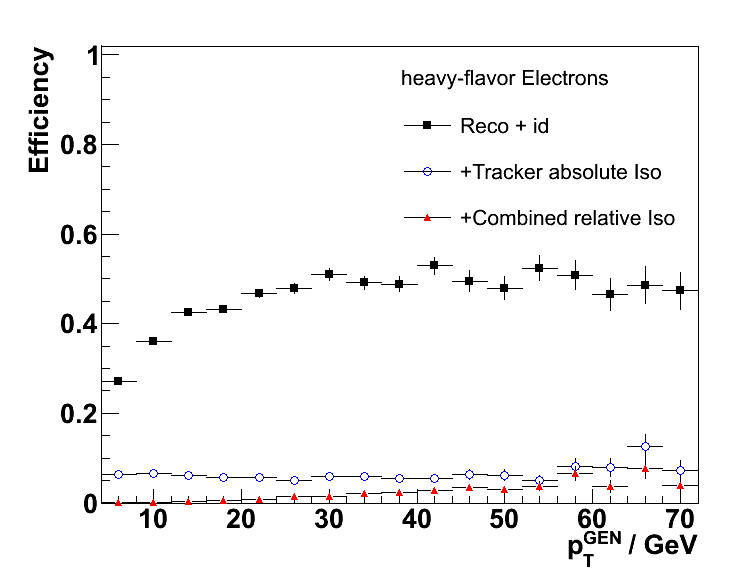
\includegraphics[scale=0.32]{./plots/hadron_ele_eff.png}}
\end{minipage}
\caption{\textit{Electron reconstruction and isolation efficiencies as a function of the generated electron $p_{T}$, for prompt electrons (left) and electrons from heavy-flavor decays (right). } }
\label{fig:ele-eff}
\end{figure}

\begin{figure}[h!]
\begin{minipage}[b]{0.5\linewidth}
\centering
{\label{fig:lm1_cor}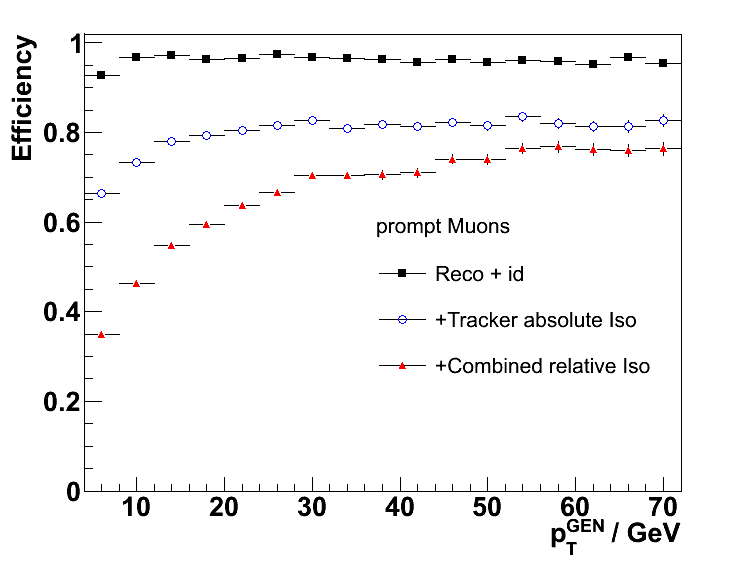
\includegraphics[scale=0.32]{./plots/prompt_muon_eff.png}}
\end{minipage}
\begin{minipage}[b]{0.5\linewidth}
\centering
{\label{fig:qcd_cor}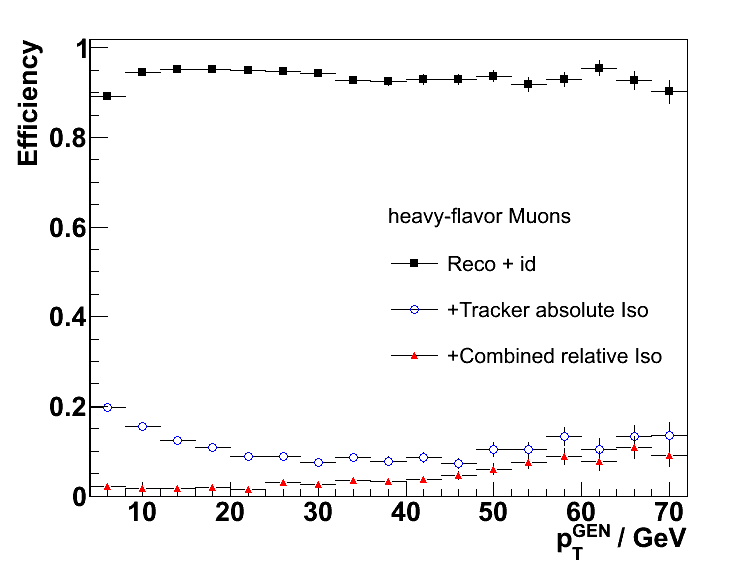
\includegraphics[scale=0.32]{./plots/hadron_muon_eff.png}}
\end{minipage}
\caption{\textit{Muon reconstruction and isolation efficiencies as a function of the generated muon $p_{T}$, for prompt muons (left) and muons from heavy-flavor decays (right). } }
\label{fig:muon-eff}
\end{figure}

\subsection{Physics objects cross cleaning}

Additional ``isolation-like'' requirements are imposed to the leptons and jets of the analysis, with the objective of resolving ambiguities between overlapping objects. In general, it is quite usual in the reconstruction, that some low-level detector information (e.g. energy deposit in the calorimeters) is shared between different candidate objects. In many of the cases, this effect may result in duplication of the energy, which in turn distroits the overall energy balancing in the event. Therefore, one needs to apply an object cleaning across different collections of reconstructed candidates (electrons, muons, jets etc). 

For the current analysis, it is vital to apply an electron-jet cleaning, so that not to count an isolated electron as an additional (fake) jet which appears in the jet collection. Furthermore, a muon-jet cross-cleaning is necessary to correct for the energy in jets taken by a (non-isolated) muon, in the heavy-flavor decays. The overall cleaning requirements are based on whether the electron or muon is isolated or not. In short, the following cross-cleaning steps have been applied: \\

\noindent \textbf{Electron-jet cross cleaning}: for each electron passing the ID criteria, the shared energy between the electron and its closest jet (within $\Delta R = 0.5$) is calculated, based on the electronmagnetic energy in towers shared by the two objects. If the electron is isolated, the shared energy is subtracted from the jet, and both objects are kept in the event. If, however, the ratio of shared energy to electron energy is above a threshold (0.7), then the jet is completely removed. If the electron is non-isolated and the shared energy is above a threshold, then the electron is removed and its energy minus the shared energy added vectorially to the jet. All other electrons, not passing the ID requirements and having an overlap with a jet, are rejected from the event.

\noindent \textbf{Muon-jet cross cleaning}: only muons passing the quality and identification criteria are considered. If the muon is not isolated and within a $\Delta R < 0.5$ from a jet, then the muon is dropped and its energy is added vectorially to the jet.

Other cross-cleaning procedures between different combinations of collections are applied such as: photon-jet cross-cleaning, with similar considerations as in the electron-jet case, as well as electron-photon cross-cleaning in order to remove fake photons originating from electrons.

\begin{comment}

\nonindent \textbf{Electron-jet cross cleaning}: if an isolated electron is found close to a jet (with EMF$<0.9$), i.e. $\Delta R (\textrm{e-Jet}) < 0.5$, and within a cone of 0.5, then the event is considered to be ambiguous and it is vetoed. If there is a non-isolated electron found in the event, then this is rejected if it has $p_{T} < 30$~GeV\footnote{In general, a non-isolated electron is most likely a fake electron, originating from a jet. For low $p_{T}$ non-isolated electrons, the source jet is also on average of low $p_{T}$ which may have been rejected by the jet energy threshold requirement.}. In all other cases ($p_{T}^{e} > 30$~GeV), the electron is rejected if it is found within a jet ($\Delta R(\textrm{non-iso e - Jet}) < 0.5$) - electron is included in the jet -, or otherwise, the whole event is vetoed ($\Delta R (\textrm{non-iso e - Jet}) > 0.5$).  \\

\noindent \textbf{Muon-jet cross cleaning}:

\end{comment}

%\end{itemize}


%\subsection{Event cleaning and kinematics}
